\documentclass[]{article}
\usepackage{lmodern}
\usepackage{amssymb,amsmath}
\usepackage{ifxetex,ifluatex}
\usepackage{fixltx2e} % provides \textsubscript
\ifnum 0\ifxetex 1\fi\ifluatex 1\fi=0 % if pdftex
  \usepackage[T1]{fontenc}
  \usepackage[utf8]{inputenc}
\else % if luatex or xelatex
  \ifxetex
    \usepackage{mathspec}
  \else
    \usepackage{fontspec}
  \fi
  \defaultfontfeatures{Ligatures=TeX,Scale=MatchLowercase}
\fi
% use upquote if available, for straight quotes in verbatim environments
\IfFileExists{upquote.sty}{\usepackage{upquote}}{}
% use microtype if available
\IfFileExists{microtype.sty}{%
\usepackage{microtype}
\UseMicrotypeSet[protrusion]{basicmath} % disable protrusion for tt fonts
}{}
\usepackage[margin=1in]{geometry}
\usepackage{hyperref}
\hypersetup{unicode=true,
            pdftitle={Homework 1},
            pdfauthor={PSTAT 131/231, Winter 2019},
            pdfborder={0 0 0},
            breaklinks=true}
\urlstyle{same}  % don't use monospace font for urls
\usepackage{color}
\usepackage{fancyvrb}
\newcommand{\VerbBar}{|}
\newcommand{\VERB}{\Verb[commandchars=\\\{\}]}
\DefineVerbatimEnvironment{Highlighting}{Verbatim}{commandchars=\\\{\}}
% Add ',fontsize=\small' for more characters per line
\usepackage{framed}
\definecolor{shadecolor}{RGB}{248,248,248}
\newenvironment{Shaded}{\begin{snugshade}}{\end{snugshade}}
\newcommand{\KeywordTok}[1]{\textcolor[rgb]{0.13,0.29,0.53}{\textbf{#1}}}
\newcommand{\DataTypeTok}[1]{\textcolor[rgb]{0.13,0.29,0.53}{#1}}
\newcommand{\DecValTok}[1]{\textcolor[rgb]{0.00,0.00,0.81}{#1}}
\newcommand{\BaseNTok}[1]{\textcolor[rgb]{0.00,0.00,0.81}{#1}}
\newcommand{\FloatTok}[1]{\textcolor[rgb]{0.00,0.00,0.81}{#1}}
\newcommand{\ConstantTok}[1]{\textcolor[rgb]{0.00,0.00,0.00}{#1}}
\newcommand{\CharTok}[1]{\textcolor[rgb]{0.31,0.60,0.02}{#1}}
\newcommand{\SpecialCharTok}[1]{\textcolor[rgb]{0.00,0.00,0.00}{#1}}
\newcommand{\StringTok}[1]{\textcolor[rgb]{0.31,0.60,0.02}{#1}}
\newcommand{\VerbatimStringTok}[1]{\textcolor[rgb]{0.31,0.60,0.02}{#1}}
\newcommand{\SpecialStringTok}[1]{\textcolor[rgb]{0.31,0.60,0.02}{#1}}
\newcommand{\ImportTok}[1]{#1}
\newcommand{\CommentTok}[1]{\textcolor[rgb]{0.56,0.35,0.01}{\textit{#1}}}
\newcommand{\DocumentationTok}[1]{\textcolor[rgb]{0.56,0.35,0.01}{\textbf{\textit{#1}}}}
\newcommand{\AnnotationTok}[1]{\textcolor[rgb]{0.56,0.35,0.01}{\textbf{\textit{#1}}}}
\newcommand{\CommentVarTok}[1]{\textcolor[rgb]{0.56,0.35,0.01}{\textbf{\textit{#1}}}}
\newcommand{\OtherTok}[1]{\textcolor[rgb]{0.56,0.35,0.01}{#1}}
\newcommand{\FunctionTok}[1]{\textcolor[rgb]{0.00,0.00,0.00}{#1}}
\newcommand{\VariableTok}[1]{\textcolor[rgb]{0.00,0.00,0.00}{#1}}
\newcommand{\ControlFlowTok}[1]{\textcolor[rgb]{0.13,0.29,0.53}{\textbf{#1}}}
\newcommand{\OperatorTok}[1]{\textcolor[rgb]{0.81,0.36,0.00}{\textbf{#1}}}
\newcommand{\BuiltInTok}[1]{#1}
\newcommand{\ExtensionTok}[1]{#1}
\newcommand{\PreprocessorTok}[1]{\textcolor[rgb]{0.56,0.35,0.01}{\textit{#1}}}
\newcommand{\AttributeTok}[1]{\textcolor[rgb]{0.77,0.63,0.00}{#1}}
\newcommand{\RegionMarkerTok}[1]{#1}
\newcommand{\InformationTok}[1]{\textcolor[rgb]{0.56,0.35,0.01}{\textbf{\textit{#1}}}}
\newcommand{\WarningTok}[1]{\textcolor[rgb]{0.56,0.35,0.01}{\textbf{\textit{#1}}}}
\newcommand{\AlertTok}[1]{\textcolor[rgb]{0.94,0.16,0.16}{#1}}
\newcommand{\ErrorTok}[1]{\textcolor[rgb]{0.64,0.00,0.00}{\textbf{#1}}}
\newcommand{\NormalTok}[1]{#1}
\usepackage{graphicx,grffile}
\makeatletter
\def\maxwidth{\ifdim\Gin@nat@width>\linewidth\linewidth\else\Gin@nat@width\fi}
\def\maxheight{\ifdim\Gin@nat@height>\textheight\textheight\else\Gin@nat@height\fi}
\makeatother
% Scale images if necessary, so that they will not overflow the page
% margins by default, and it is still possible to overwrite the defaults
% using explicit options in \includegraphics[width, height, ...]{}
\setkeys{Gin}{width=\maxwidth,height=\maxheight,keepaspectratio}
\IfFileExists{parskip.sty}{%
\usepackage{parskip}
}{% else
\setlength{\parindent}{0pt}
\setlength{\parskip}{6pt plus 2pt minus 1pt}
}
\setlength{\emergencystretch}{3em}  % prevent overfull lines
\providecommand{\tightlist}{%
  \setlength{\itemsep}{0pt}\setlength{\parskip}{0pt}}
\setcounter{secnumdepth}{0}
% Redefines (sub)paragraphs to behave more like sections
\ifx\paragraph\undefined\else
\let\oldparagraph\paragraph
\renewcommand{\paragraph}[1]{\oldparagraph{#1}\mbox{}}
\fi
\ifx\subparagraph\undefined\else
\let\oldsubparagraph\subparagraph
\renewcommand{\subparagraph}[1]{\oldsubparagraph{#1}\mbox{}}
\fi

%%% Use protect on footnotes to avoid problems with footnotes in titles
\let\rmarkdownfootnote\footnote%
\def\footnote{\protect\rmarkdownfootnote}

%%% Change title format to be more compact
\usepackage{titling}

% Create subtitle command for use in maketitle
\newcommand{\subtitle}[1]{
  \posttitle{
    \begin{center}\large#1\end{center}
    }
}

\setlength{\droptitle}{-2em}

  \title{Homework 1}
    \pretitle{\vspace{\droptitle}\centering\huge}
  \posttitle{\par}
    \author{PSTAT 131/231, Winter 2019}
    \preauthor{\centering\large\emph}
  \postauthor{\par}
      \predate{\centering\large\emph}
  \postdate{\par}
    \date{\textbf{Due on January 26, 2018 at 11:55 pm}}

\usepackage{booktabs}
\usepackage{longtable}
\usepackage{array}
\usepackage{multirow}
\usepackage[table]{xcolor}
\usepackage{wrapfig}
\usepackage{float}
\usepackage{colortbl}
\usepackage{pdflscape}
\usepackage{tabu}
\usepackage{threeparttable}
\usepackage{threeparttablex}
\usepackage[normalem]{ulem}
\usepackage{makecell}

\begin{document}
\maketitle

\textbf{Note:} If you are working with a partner, please submit only one
homework per group with both names and whether you are taking the course
for graduate credit or not. Submit your Rmarkdown (.Rmd) and the
compiled pdf on Gauchospace.

\begin{center}\rule{0.5\linewidth}{\linethickness}\end{center}

\textbf{Predicting Algae Blooms}

\textbf{\emph{Background}} High concentrations of certain harmful algae
in rivers constitute a serious ecological problem with a strong impact
not only on river lifeforms, but also on water quality. Being able to
monitor and perform an early forecast of algae blooms is essential to
improving the quality of rivers.

With the goal of addressing this prediction problem, several water
samples were collected in different European rivers at different times
during a period of approximately 1 year. For each water sample,
different chemical properties were measured as well as the frequency of
occurrence of seven harmful algae. Some other characteristics of the
water collection process were also stored, such as the season of the
year, the river size, and the river speed.

\textbf{\emph{Goal}} We want to understand how these frequencies are
related to certain chemical attributes of water samples as well as other
characteristics of the samples (like season of the year, type of river,
etc.)

\textbf{\emph{Data Description}} The data set consists of data for 200
water samples and each observation in the available datasets is in
effect an aggregation of several water samples collected from the same
river over a period of 3 months, during the same season of the year.
Each observation contains information on 11 variables. Three of these
variables are nominal and describe the season of the year when the water
samples to be aggregated were collected, as well as the size and speed
of the river in question. The eight remaining variables are values of
different chemical parameters measured in the water samples forming the
aggregation, namely: Maximum pH value, Minimum value of \(O_2\)
(oxygen), Mean value of Cl (chloride), Mean value of \(NO_3^-\)
(nitrates), Mean value of \(NH_4^+\) (ammonium), Mean of \(PO^{3}_4\)
(orthophosphate), Mean of total \(PO_4\) (phosphate) and Mean of
chlorophyll.

Associated with each of these parameters are seven frequency numbers of
different harmful algae found in the respective water samples. No
information is given regarding the names of the algae that were
identified.

We can start the analysis by loading into R the data from the
``algaeBloom.txt'' file (the training data, i.e.~the data that will be
used to obtain the predictive models). To read the data from the file it
is sufficient to issue the following command:

\begin{Shaded}
\begin{Highlighting}[]
\NormalTok{algae <-}\StringTok{ }\KeywordTok{read_table2}\NormalTok{(}\StringTok{"algaeBloom.txt"}\NormalTok{, }\DataTypeTok{col_names=}
                      \KeywordTok{c}\NormalTok{(}\StringTok{'season'}\NormalTok{,}\StringTok{'size'}\NormalTok{,}\StringTok{'speed'}\NormalTok{,}\StringTok{'mxPH'}\NormalTok{,}\StringTok{'mnO2'}\NormalTok{,}\StringTok{'Cl'}\NormalTok{,}\StringTok{'NO3'}\NormalTok{,}\StringTok{'NH4'}\NormalTok{,}
                        \StringTok{'oPO4'}\NormalTok{,}\StringTok{'PO4'}\NormalTok{,}\StringTok{'Chla'}\NormalTok{,}\StringTok{'a1'}\NormalTok{,}\StringTok{'a2'}\NormalTok{,}\StringTok{'a3'}\NormalTok{,}\StringTok{'a4'}\NormalTok{,}\StringTok{'a5'}\NormalTok{,}\StringTok{'a6'}\NormalTok{,}\StringTok{'a7'}\NormalTok{), }
                      \DataTypeTok{na=}\StringTok{"XXXXXXX"}\NormalTok{)}

\KeywordTok{glimpse}\NormalTok{(algae)}
\end{Highlighting}
\end{Shaded}

\begin{enumerate}
\def\labelenumi{\arabic{enumi}.}
\item
  \textbf{\emph{Descriptive summary statistics}} Given the lack of
  further information on the problem domain, it is wise to investigate
  some of the statistical properties of the data, so as to get a better
  grasp of the problem. It is always a good idea to start our analysis
  with some kind of exploratory data analysis. A first idea of the
  statistical properties of the data can be obtained through a summary
  of its descriptive statistics.

  \begin{enumerate}
  \tightlist
  \item
    Count the number of observations in each season using
    \texttt{summarise()} in \texttt{dplyr}.
  \end{enumerate}
\end{enumerate}

\begin{Shaded}
\begin{Highlighting}[]
\NormalTok{season_obs <-}\StringTok{ }\NormalTok{algae }\OperatorTok\StringTok{ }
\StringTok{  }\KeywordTok{count}\NormalTok{(}\StringTok{"season"}\NormalTok{)}

\NormalTok{season_obs}
\end{Highlighting}
\end{Shaded}

\begin{verbatim}
##   season freq
## 1 autumn   40
## 2 spring   53
## 3 summer   45
## 4 winter   62
\end{verbatim}

There are 40 observations in autumn, 53 in spring, 45 in summer, and 62
in winter.

\begin{verbatim}
#. Are there missing values? Calculate the mean and variance of each
chemical (Ignore $a_1$ through $a_7$). What do you notice about the
magnitude of the two quantities for different chemicals? 
\end{verbatim}

\begin{Shaded}
\begin{Highlighting}[]
\NormalTok{algae_na <-}\StringTok{ }\NormalTok{algae }\OperatorTok
\StringTok{  }\KeywordTok{select}\NormalTok{(}\KeywordTok{c}\NormalTok{(}\StringTok{'mxPH'}\NormalTok{,}\StringTok{'mnO2'}\NormalTok{,}\StringTok{'Cl'}\NormalTok{,}\StringTok{'NO3'}\NormalTok{,}\StringTok{'NH4'}\NormalTok{, }\StringTok{'oPO4'}\NormalTok{,}\StringTok{'PO4'}\NormalTok{,}\StringTok{'Chla'}\NormalTok{)) }\OperatorTok
\StringTok{  }\KeywordTok{summarise_all}\NormalTok{(}\ControlFlowTok{function}\NormalTok{(x) }\KeywordTok{sum}\NormalTok{(}\KeywordTok{is.na}\NormalTok{(x)))}
\end{Highlighting}
\end{Shaded}

There are missing values for several variables. One value is missing for
mxPH. NO3, NH4, oPO4, and PO4 are all missing two values. Cl and Chla
are each missing 10 and 12 variables.

\begin{Shaded}
\begin{Highlighting}[]
\KeywordTok{print}\NormalTok{(}\StringTok{'Mean'}\NormalTok{)}
\end{Highlighting}
\end{Shaded}

\begin{verbatim}
## [1] "Mean"
\end{verbatim}

\begin{Shaded}
\begin{Highlighting}[]
\NormalTok{chem_means <-}\StringTok{ }\NormalTok{algae }\OperatorTok\StringTok{ }
\StringTok{  }\KeywordTok{select}\NormalTok{(}\KeywordTok{c}\NormalTok{(}\StringTok{'mxPH'}\NormalTok{,}\StringTok{'mnO2'}\NormalTok{,}\StringTok{'Cl'}\NormalTok{,}\StringTok{'NO3'}\NormalTok{,}\StringTok{'NH4'}\NormalTok{, }\StringTok{'oPO4'}\NormalTok{,}\StringTok{'PO4'}\NormalTok{,}\StringTok{'Chla'}\NormalTok{)) }\OperatorTok
\StringTok{  }\KeywordTok{summarise_all}\NormalTok{(}\ControlFlowTok{function}\NormalTok{ (x) }\KeywordTok{mean}\NormalTok{(x, }\DataTypeTok{na.rm=}\OtherTok{TRUE}\NormalTok{)) }

\KeywordTok{print}\NormalTok{(}\StringTok{'Variance'}\NormalTok{)}
\end{Highlighting}
\end{Shaded}

\begin{verbatim}
## [1] "Variance"
\end{verbatim}

\begin{Shaded}
\begin{Highlighting}[]
\NormalTok{chem_vars <-}\StringTok{ }\NormalTok{algae }\OperatorTok\StringTok{ }
\StringTok{   }\KeywordTok{select}\NormalTok{(}\KeywordTok{c}\NormalTok{(}\StringTok{'mxPH'}\NormalTok{,}\StringTok{'mnO2'}\NormalTok{,}\StringTok{'Cl'}\NormalTok{,}\StringTok{'NO3'}\NormalTok{,}\StringTok{'NH4'}\NormalTok{, }\StringTok{'oPO4'}\NormalTok{,}\StringTok{'PO4'}\NormalTok{,}\StringTok{'Chla'}\NormalTok{)) }\OperatorTok
\StringTok{  }\KeywordTok{summarise_all}\NormalTok{(}\ControlFlowTok{function}\NormalTok{ (x) }\KeywordTok{var}\NormalTok{(x, }\DataTypeTok{na.rm=}\OtherTok{TRUE}\NormalTok{)) }

\NormalTok{var_mean_ratio <-}\StringTok{ }\NormalTok{chem_vars}\OperatorTok{/}\NormalTok{chem_means}
\end{Highlighting}
\end{Shaded}

The mean for NH4 is the largest, but it had a disproportionately large
variance in observed measurements that resulted in this chemical having
the largest variance to mean ratio at 7,683. PO4 had the second highest
variance to mean ratio 120 followed by oPO4's variance to mean ratio of
112. These results highlight considerable variation among the measured
values for NH4, PO4, and oPO4, which could be attributed to seasonal
variation in uptake of these critical nutrients for algae that are more
active in warmer temperatures but tend to die off in the winter. The
mxPH had the smallest variance and the smallest variance to mean ratio
of 0.04, which demonstrates consistency of maximum pH observed across
the sample sites and seasons.

\begin{verbatim}
#. Mean and Variance is one measure of central tendency and spread of data.
Median and Median Absolute Deviation are alternative measures of central
tendency and spread. 

    For a univariate data set $X_1, X_2, ..., X_n$, the Median Absolute Deviation (MAD) is defined as the median of the absolute deviations from the data's median: $$\text{MAD}=\text{median} (|X_i-\text{median}(X)|)$$

    Compute median and MAD of each chemical and compare the two sets of quantities (i.e., mean & variance vs. median & MAD). What do you notice? 
    
\end{verbatim}

\begin{Shaded}
\begin{Highlighting}[]
\KeywordTok{print}\NormalTok{(}\StringTok{'Median'}\NormalTok{)}
\end{Highlighting}
\end{Shaded}

\begin{verbatim}
## [1] "Median"
\end{verbatim}

\begin{Shaded}
\begin{Highlighting}[]
\NormalTok{chem_medians <-}\StringTok{ }\NormalTok{algae }\OperatorTok\StringTok{ }
\StringTok{  }\KeywordTok{select}\NormalTok{(}\KeywordTok{c}\NormalTok{(}\StringTok{'mxPH'}\NormalTok{,}\StringTok{'mnO2'}\NormalTok{,}\StringTok{'Cl'}\NormalTok{,}\StringTok{'NO3'}\NormalTok{,}\StringTok{'NH4'}\NormalTok{, }\StringTok{'oPO4'}\NormalTok{,}\StringTok{'PO4'}\NormalTok{,}\StringTok{'Chla'}\NormalTok{)) }\OperatorTok\StringTok{ }
\StringTok{  }\KeywordTok{summarise_all}\NormalTok{(}\ControlFlowTok{function}\NormalTok{ (x) }\KeywordTok{median}\NormalTok{(x, }\DataTypeTok{na.rm=}\OtherTok{TRUE}\NormalTok{))}

\KeywordTok{print}\NormalTok{(}\StringTok{'MADs'}\NormalTok{)}
\end{Highlighting}
\end{Shaded}

\begin{verbatim}
## [1] "MADs"
\end{verbatim}

\begin{Shaded}
\begin{Highlighting}[]
\NormalTok{chem_mads <-}\StringTok{ }\NormalTok{algae }\OperatorTok\StringTok{ }
\StringTok{  }\KeywordTok{select}\NormalTok{(}\KeywordTok{c}\NormalTok{(}\StringTok{'mxPH'}\NormalTok{,}\StringTok{'mnO2'}\NormalTok{,}\StringTok{'Cl'}\NormalTok{,}\StringTok{'NO3'}\NormalTok{,}\StringTok{'NH4'}\NormalTok{, }\StringTok{'oPO4'}\NormalTok{,}\StringTok{'PO4'}\NormalTok{,}\StringTok{'Chla'}\NormalTok{)) }\OperatorTok
\StringTok{  }\KeywordTok{summarise_all}\NormalTok{(}\ControlFlowTok{function}\NormalTok{ (x) }\KeywordTok{mad}\NormalTok{(x, }\DataTypeTok{na.rm=}\OtherTok{TRUE}\NormalTok{))}

\NormalTok{mads_medians_ratio <-}\StringTok{ }\NormalTok{chem_mads}\OperatorTok{/}\NormalTok{chem_medians}
\end{Highlighting}
\end{Shaded}

The ratio of MAD to median for all chemicals except mxPH are smaller in
magnitude than the variance to mean ratio for each parameter,
respectively. For most parameters, the MAD to median was many times
smaller, and in the case of NH4 there was a reduction of three orders of
magnitude as compared to its variance to mean ratio. PO4 and oPO4 MAD to
median ratios were two orders of magnitude smaler than variance to mean
ratios. These results highlight the significant difference between the
results presented through two methods of central tendency. The
considerably lower MAD to median ratios demonstrates that a few outlier
measurements may be causing much higher variance in the calculation of
means while the calculation of MAD will not be severely influenced by
outliers because the MAD is the median of the absolute difference
between each measurement and the mediant of the measurements.Bearing
this in mind, it is important to consider what an appropriate
representation of central tendency is and determine whether or not
particular measures truly are outliers or not.

\begin{enumerate}
\def\labelenumi{\arabic{enumi}.}
\setcounter{enumi}{1}
\item
  \textbf{\emph{Data visualization}} Most of the time, the information
  in the data set is also well captured graphically. Histogram, scatter
  plot, boxplot, Q-Q plot are frequently used tools for data
  visualization. Use ggplot for all of these visualizations.

  \begin{enumerate}
  \tightlist
  \item
    Produce a histogram of \(mxPH\) with the title `Histogram of mxPH'
    based on algae data set. Use an appropriate argument to show the
    probability instead of the frequency as the vertical axis. (Hint:
    look at the examples in the help file for function
    \texttt{geom\_histogram()}). Is the distribution skewed?
  \end{enumerate}
\end{enumerate}

\begin{Shaded}
\begin{Highlighting}[]
\NormalTok{hist_mxPH <-}\StringTok{ }\KeywordTok{ggplot}\NormalTok{(algae, }\KeywordTok{aes}\NormalTok{(}\DataTypeTok{x =}\NormalTok{ mxPH)) }\OperatorTok{+}
\StringTok{  }\KeywordTok{geom_histogram}\NormalTok{(}\DataTypeTok{bins =} \DecValTok{12}\NormalTok{)  }\OperatorTok{+}\StringTok{ }\CommentTok{#2*(200)^1/3}
\StringTok{  }\KeywordTok{labs}\NormalTok{(}\DataTypeTok{title =} \StringTok{'Histogram of mxPH'}\NormalTok{) }\OperatorTok{+}
\StringTok{  }\KeywordTok{ylab}\NormalTok{(}\StringTok{'Probability'}\NormalTok{) }\OperatorTok{+}
\StringTok{  }\KeywordTok{scale_y_continuous}\NormalTok{(}\DataTypeTok{labels =}\NormalTok{scales}\OperatorTok{::}\NormalTok{percent) }\OperatorTok{+}
\StringTok{  }\KeywordTok{geom_density}\NormalTok{() }\OperatorTok{+}
\StringTok{  }\KeywordTok{geom_rug}\NormalTok{()}

\NormalTok{hist_mxPH}
\end{Highlighting}
\end{Shaded}

\begin{verbatim}
## Warning: Removed 1 rows containing non-finite values (stat_bin).
\end{verbatim}

\begin{verbatim}
## Warning: Removed 1 rows containing non-finite values (stat_density).
\end{verbatim}

\begin{center}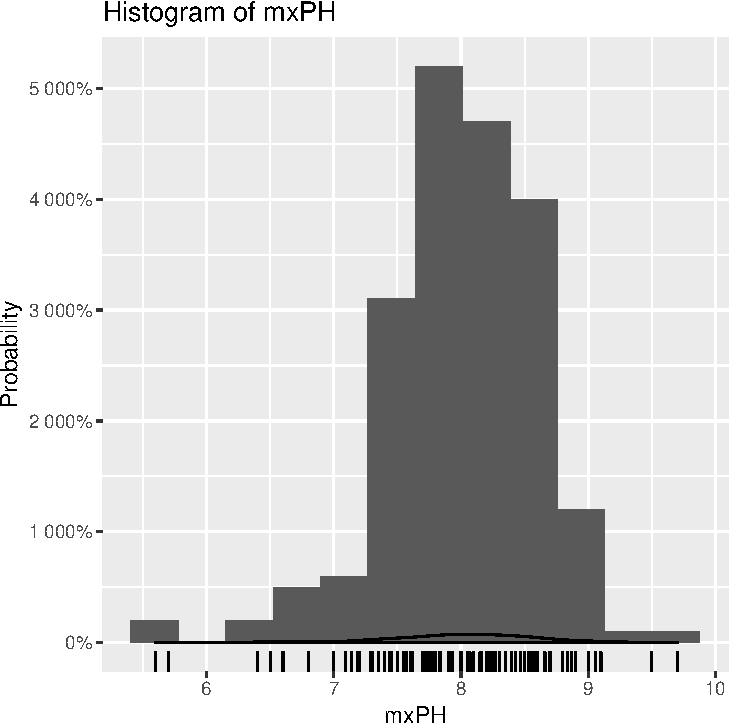
\includegraphics{homework1-handout_files/figure-latex/unnamed-chunk-1-1} \end{center}

The histogram of mxPH is skewed with several more observations in the
three bins immediately greater than the mean as compared to the three
bins just below the mean.

\begin{verbatim}
#. Add a density curve using `geom_density()` and rug plots using `geom_rug()` to above histogram. 

#. Create a boxplot with the title 'A conditioned Boxplot of Algal $a_1$' for $a_1$ grouped by $size$. (Refer to help page for `geom_boxplot()`). 
\end{verbatim}

\begin{Shaded}
\begin{Highlighting}[]
\NormalTok{algae_boxplot <-}\StringTok{ }\KeywordTok{ggplot}\NormalTok{(algae, }\KeywordTok{aes}\NormalTok{(size, a1)) }\OperatorTok{+}
\StringTok{  }\KeywordTok{geom_boxplot}\NormalTok{(}\DataTypeTok{outlier.color =} \StringTok{'orange'}\NormalTok{) }\OperatorTok{+}
\StringTok{  }\KeywordTok{labs}\NormalTok{(}\DataTypeTok{title =} \StringTok{'A conditioned Boxplot of Algal a1'}\NormalTok{)}

\NormalTok{algae_boxplot}
\end{Highlighting}
\end{Shaded}

\begin{center}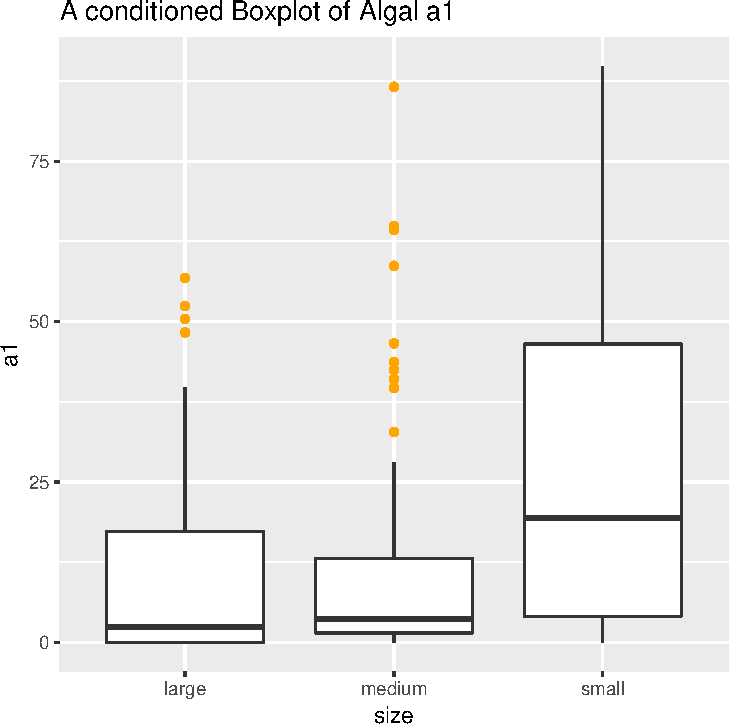
\includegraphics{homework1-handout_files/figure-latex/boxplot-1} \end{center}

\begin{enumerate}
\tightlist
\item
  Are there any outliers for \(NO3\) and \(NH4\)? How many observations
  would you consider as outliers? How did you arrive at this conclusion?
\end{enumerate}

\begin{Shaded}
\begin{Highlighting}[]
\NormalTok{NO3_boxplot <-}\StringTok{ }\KeywordTok{ggplot}\NormalTok{(algae, }\KeywordTok{aes}\NormalTok{(}\DataTypeTok{x =} \StringTok{'NO3'}\NormalTok{, }\DataTypeTok{y =}\NormalTok{ NO3)) }\OperatorTok{+}\StringTok{ }
\StringTok{  }\KeywordTok{geom_boxplot}\NormalTok{(}\DataTypeTok{outlier.color =} \StringTok{'orange'}\NormalTok{) }\OperatorTok{+}
\StringTok{  }\KeywordTok{labs}\NormalTok{(}\DataTypeTok{title =} \StringTok{'A conditioned Boxplot of NO3'}\NormalTok{)}

\NormalTok{NO3_boxplot }
\end{Highlighting}
\end{Shaded}

\begin{verbatim}
## Warning: Removed 2 rows containing non-finite values (stat_boxplot).
\end{verbatim}

\begin{center}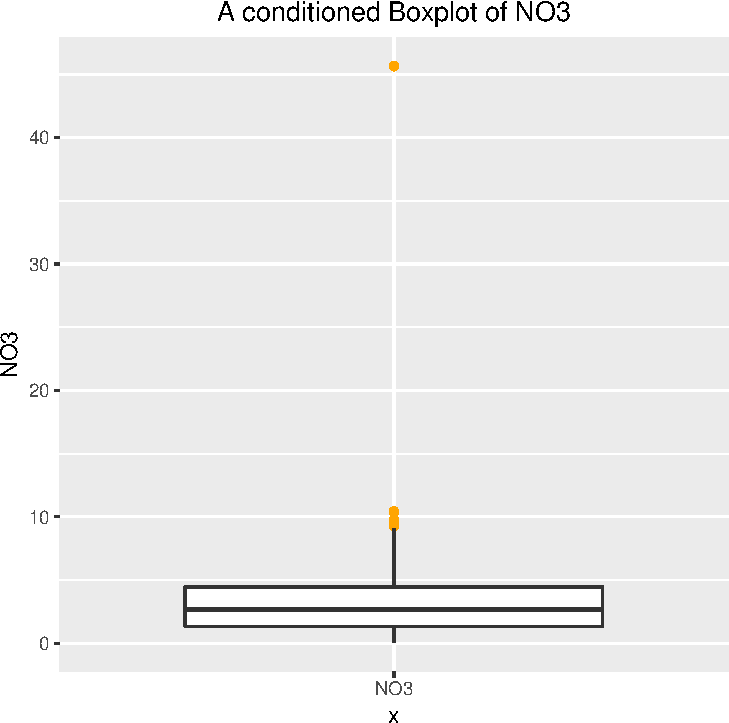
\includegraphics{homework1-handout_files/figure-latex/unnamed-chunk-2-1} \end{center}

\begin{Shaded}
\begin{Highlighting}[]
\NormalTok{NO3season_boxplot <-}\StringTok{ }\KeywordTok{ggplot}\NormalTok{(algae, }\KeywordTok{aes}\NormalTok{(season, }\DataTypeTok{y =}\NormalTok{ NO3)) }\OperatorTok{+}
\StringTok{  }\KeywordTok{geom_boxplot}\NormalTok{(}\DataTypeTok{outlier.color =} \StringTok{'orange'}\NormalTok{) }\OperatorTok{+}
\StringTok{  }\KeywordTok{labs}\NormalTok{(}\DataTypeTok{title =} \StringTok{'A conditioned Boxplot of NO3 by Season'}\NormalTok{)}

\NormalTok{NO3season_boxplot}
\end{Highlighting}
\end{Shaded}

\begin{verbatim}
## Warning: Removed 2 rows containing non-finite values (stat_boxplot).
\end{verbatim}

\begin{center}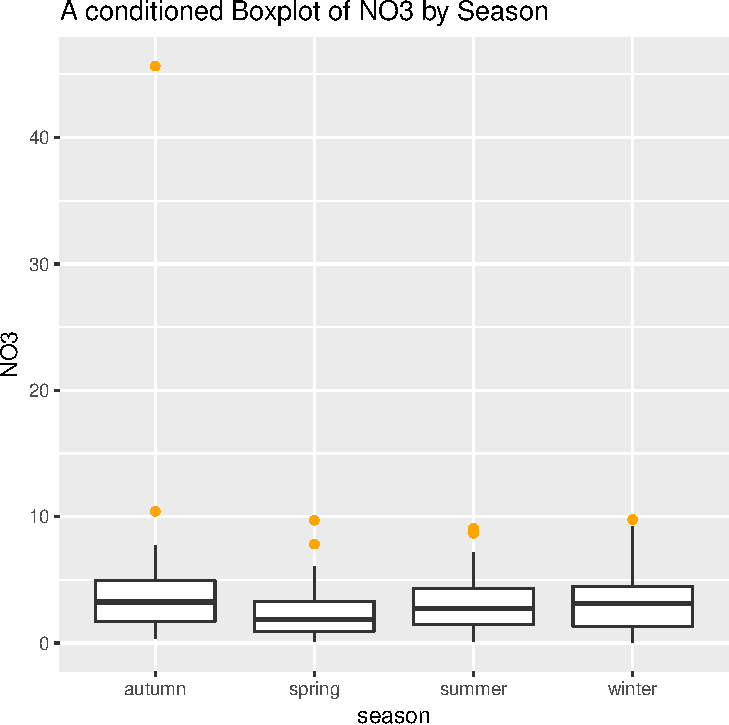
\includegraphics{homework1-handout_files/figure-latex/unnamed-chunk-2-2} \end{center}

By separating the NO3 data into seasons, we can see that there is a
clear outlier in autumn that is significantly further from the
Interquartile Range than outliers at more than four times the value
measured for NO3 in other months. Note: outliers are indicated in
orange. Thus, we will only consider this one autumn outlier as a true
outlier.

\begin{Shaded}
\begin{Highlighting}[]
\NormalTok{NH4_boxplot <-}\StringTok{ }\KeywordTok{ggplot}\NormalTok{(algae, }\KeywordTok{aes}\NormalTok{(}\DataTypeTok{x =} \StringTok{'NH4'}\NormalTok{, }\DataTypeTok{y =}\NormalTok{ NH4)) }\OperatorTok{+}\StringTok{ }
\StringTok{  }\KeywordTok{geom_boxplot}\NormalTok{(}\DataTypeTok{outlier.color =} \StringTok{'orange'}\NormalTok{) }\OperatorTok{+}
\StringTok{  }\KeywordTok{labs}\NormalTok{(}\DataTypeTok{title =} \StringTok{'A conditioned Boxplot of NH4'}\NormalTok{)}

\NormalTok{NH4_boxplot }
\end{Highlighting}
\end{Shaded}

\begin{verbatim}
## Warning: Removed 2 rows containing non-finite values (stat_boxplot).
\end{verbatim}

\begin{center}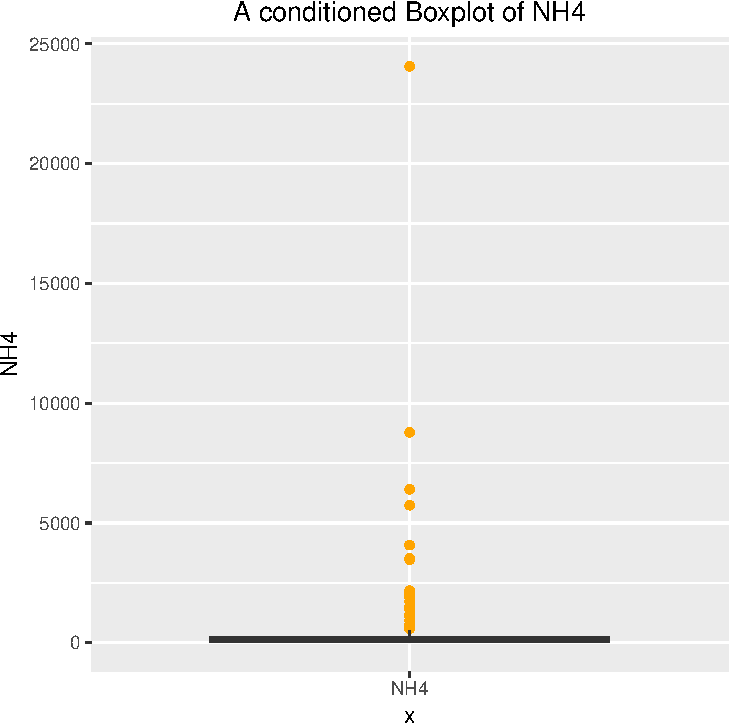
\includegraphics{homework1-handout_files/figure-latex/unnamed-chunk-3-1} \end{center}

\begin{Shaded}
\begin{Highlighting}[]
\NormalTok{NH4season_boxplot <-}\StringTok{ }\KeywordTok{ggplot}\NormalTok{(algae, }\KeywordTok{aes}\NormalTok{(season, }\DataTypeTok{y =}\NormalTok{ NH4)) }\OperatorTok{+}
\StringTok{  }\KeywordTok{geom_boxplot}\NormalTok{(}\DataTypeTok{outlier.color =} \StringTok{'orange'}\NormalTok{) }\OperatorTok{+}
\StringTok{  }\KeywordTok{labs}\NormalTok{(}\DataTypeTok{title =} \StringTok{'A conditioned Boxplot of NH4 by Season'}\NormalTok{)}

\NormalTok{NH4season_boxplot}
\end{Highlighting}
\end{Shaded}

\begin{verbatim}
## Warning: Removed 2 rows containing non-finite values (stat_boxplot).
\end{verbatim}

\begin{center}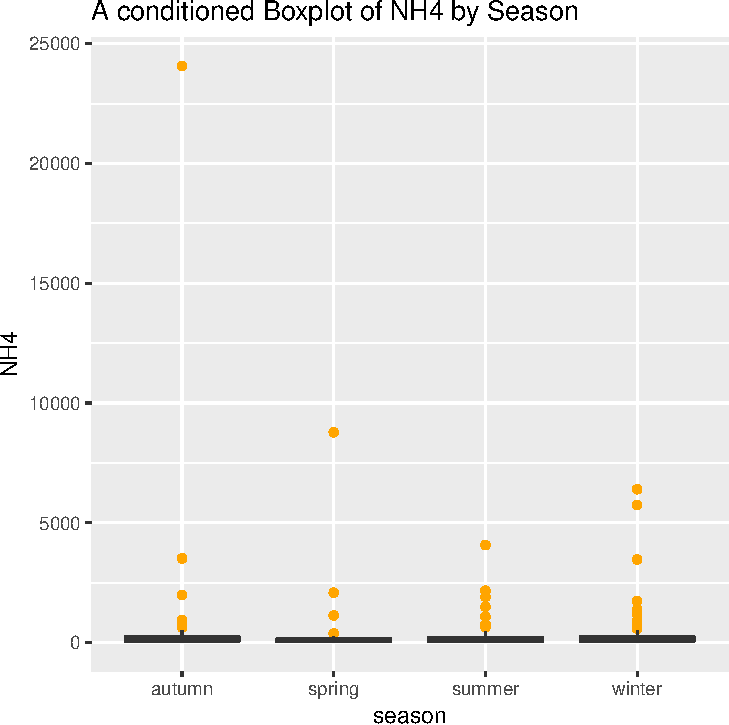
\includegraphics{homework1-handout_files/figure-latex/unnamed-chunk-3-2} \end{center}

Determining the number of outliers for NH4 measurements is slightly more
challenging, but splitting up the box plot into seasonal observations
helps once again. There are four clear true outliers across all seasons
(one in both autumn and summer, two in winter) with values above the
5000 threshold that are well beyond the range of other measurements. It
also seems reasonable to count the three outlier points (one in each of
autumn, summer and winter) above the \textasciitilde{}3000 value
threshold as additional true outliers. While this is a somewhat
arbitrary threshold, these three points seemed similarly distinct from
the other outlier points closer to the extent of the Interquartile
Range. However, it is possible that the presence of these three measures
of NH4 at \textasciitilde{}3000 across three seasons may suggest that
this is not an outlier but a characteristic of the study site. The
remaining outlier points below NH4 = 2500 are not considered true
outliers because they are not too far beyond the Interquartile Range for
each season and it would be challenging to tease out any further
groupings to distinguish some of these points from others as ture
outliers. Thus a total of seven true outliers were chose for NH4
observations.

\begin{verbatim}
#. Compare mean & variance vs. median & MAD for $NO3$ and $NH4$. What do you notice? Can you conclude which set of measures is more robust when outliers are present? 
\end{verbatim}

There is a larger difference between mean and median values for NH4 than
NO3. The same pattern is true for variance and MAD, however the variance
is much larger for NH4 than NO3. The median and MAD are a more
appropriate measure when outliers are present because averaging with
outliers can skew the calculation as was the case with one autumn
measure of both NO3 and NH4. The outliers identified for NH4
measurements in other seasons similarly would skew the mean of this
parameter.

\begin{center}\rule{0.5\linewidth}{\linethickness}\end{center}

\textbf{Predicting Algae Blooms}

Some water samples contained unknown values in several chemicals.
Missing data are very common in real-world problems, and may prevent the
use of certain data mining techniques that are not able to handle
missing values.

In this homework, we are going to introduce various ways to deal with
missing values. After all the missing values have been taken care of, we
will build a model to investigate the relationship between the variable
\texttt{a1} and other 11 predictors (\texttt{season}, \texttt{size},
\texttt{speed}, \texttt{mxPH}, \texttt{mnO2}, \texttt{Cl}, \texttt{NO3},
\texttt{NH4}, \texttt{oPO4}, \texttt{PO4}, \texttt{Chla}) utilizing
cross-validation in the next problem.

\textbf{\emph{Dealing with missing values}}

\begin{enumerate}
\def\labelenumi{\arabic{enumi}.}
\setcounter{enumi}{2}
\item
  \begin{enumerate}
  \tightlist
  \item
    How many observations contain missing values? How many missing
    values are there in each variable?
  \end{enumerate}
\end{enumerate}

\begin{Shaded}
\begin{Highlighting}[]
\NormalTok{missingvalues <-}\StringTok{ }\NormalTok{algae }\OperatorTok
\StringTok{  }\KeywordTok{select}\NormalTok{(}\KeywordTok{c}\NormalTok{(}\StringTok{'season'}\NormalTok{,}\StringTok{'size'}\NormalTok{,}\StringTok{'speed'}\NormalTok{,}\StringTok{'mxPH'}\NormalTok{,}\StringTok{'mnO2'}\NormalTok{,}\StringTok{'Cl'}\NormalTok{,}\StringTok{'NO3'}\NormalTok{,}\StringTok{'NH4'}\NormalTok{,}
  \StringTok{'oPO4'}\NormalTok{,}\StringTok{'PO4'}\NormalTok{,}\StringTok{'Chla'}\NormalTok{,}\StringTok{'a1'}\NormalTok{,}\StringTok{'a2'}\NormalTok{,}\StringTok{'a3'}\NormalTok{,}\StringTok{'a4'}\NormalTok{,}\StringTok{'a5'}\NormalTok{, }\StringTok{'a6'}\NormalTok{, }\StringTok{'a7'}\NormalTok{)) }\OperatorTok
\StringTok{  }\KeywordTok{summarise_all}\NormalTok{(}\ControlFlowTok{function}\NormalTok{(x) }\KeywordTok{sum}\NormalTok{(}\KeywordTok{is.na}\NormalTok{(x)))}
\end{Highlighting}
\end{Shaded}

There are 16 observations that contain at least one missing value for a
parameter with a total of 33 missing variable values across all of the
observations. There is one missing value for mxPH, and two missing for
each of mnO2, NO3, NH4, oPO4, and PO4. Ten values are missing for Cl and
12 are missing for Chla.

\begin{verbatim}
#. **Removing observations with missing values**: use `filter()` function
in `dplyr` package to observations with any missing value, and save the
resulting dataset (without missing values) as `algae.del`. Report how many
observations are in `algae.del`.

    Hint: `complete.cases()` may be useful.
\end{verbatim}

\begin{Shaded}
\begin{Highlighting}[]
\NormalTok{algae.del <-}\StringTok{ }\NormalTok{algae }\OperatorTok\StringTok{ }
\StringTok{  }\KeywordTok{filter_all}\NormalTok{(}\KeywordTok{all_vars}\NormalTok{(}\OperatorTok{!}\KeywordTok{is.na}\NormalTok{(.)))}
\end{Highlighting}
\end{Shaded}

There are 184 observations in algae.del

\begin{verbatim}
#. \label{imputation} **Imputing unknowns with measures of central
tendency**: the simplest and fastest way of filling in (imputing) missing
values is to use some measures of central tendency such as mean, median and
mode.
    
    Use `mutate_at()` and `ifelse()` in `dplyr` to fill in missing values
    for each chemical with its median, and save the imputed dataset as
    `algae.med`. Report the number of observations in `algae.med`.  Display
    the values of each chemical for the $48^{th}$, $62^{th}$ and $199^{th}$
    obsevation in `algae.med`. 
\end{verbatim}

\begin{Shaded}
\begin{Highlighting}[]
\NormalTok{algae.med <-}\StringTok{ }\NormalTok{algae }\OperatorTok\StringTok{ }
\StringTok{  }\KeywordTok{mutate_at}\NormalTok{(}\DataTypeTok{.vars =} \KeywordTok{c}\NormalTok{(}\StringTok{'mxPH'}\NormalTok{,}\StringTok{'mnO2'}\NormalTok{,}\StringTok{'Cl'}\NormalTok{,}\StringTok{'NO3'}\NormalTok{,}\StringTok{'NH4'}\NormalTok{,}
  \StringTok{'oPO4'}\NormalTok{,}\StringTok{'PO4'}\NormalTok{,}\StringTok{'Chla'}\NormalTok{), }\DataTypeTok{.funs =} \KeywordTok{funs}\NormalTok{(}\KeywordTok{ifelse}\NormalTok{(}\KeywordTok{is.na}\NormalTok{(.), }\KeywordTok{median}\NormalTok{(., }\DataTypeTok{na.rm =} \OtherTok{TRUE}\NormalTok{), .)))}

\NormalTok{algae.med.}\DecValTok{48}\NormalTok{ <-}\StringTok{ }\NormalTok{algae.med[}\DecValTok{48}\NormalTok{, }\DecValTok{4}\OperatorTok{:}\DecValTok{11}\NormalTok{]}
\NormalTok{algae.med.}\DecValTok{62}\NormalTok{ <-}\StringTok{ }\NormalTok{algae.med[}\DecValTok{62}\NormalTok{, }\DecValTok{4}\OperatorTok{:}\DecValTok{11}\NormalTok{]}
\NormalTok{algae.med.}\DecValTok{199}\NormalTok{ <-}\StringTok{ }\NormalTok{algae.med[}\DecValTok{199}\NormalTok{, }\DecValTok{4}\OperatorTok{:}\DecValTok{11}\NormalTok{]}

\NormalTok{algae.med.rows <-}\StringTok{ }\KeywordTok{rbind}\NormalTok{(algae.med.}\DecValTok{48}\NormalTok{, algae.med.}\DecValTok{62}\NormalTok{, algae.med.}\DecValTok{199}\NormalTok{)}
\KeywordTok{rownames}\NormalTok{(algae.med.rows) <-}\StringTok{ }\KeywordTok{c}\NormalTok{(}\StringTok{"48"}\NormalTok{, }\StringTok{"62"}\NormalTok{, }\StringTok{"199"}\NormalTok{)}
\end{Highlighting}
\end{Shaded}

\begin{verbatim}
## Warning: Setting row names on a tibble is deprecated.
\end{verbatim}

\begin{Shaded}
\begin{Highlighting}[]
\KeywordTok{kable}\NormalTok{(algae.med.rows, }\StringTok{"latex"}\NormalTok{, }\DataTypeTok{booktabs =}\NormalTok{ T, }
      \DataTypeTok{caption =} \StringTok{"Chemical Observations for Specific Rows After Imputing"}\NormalTok{) }\OperatorTok\StringTok{  }
\StringTok{      }\KeywordTok{kable_styling}\NormalTok{(}\DataTypeTok{bootstrap_options =} \StringTok{"striped"}\NormalTok{, }\DataTypeTok{full_width =}\NormalTok{ F, }\DataTypeTok{position =} \StringTok{"center"}\NormalTok{)}
\end{Highlighting}
\end{Shaded}

\begin{table}

\caption{\label{tab:unnamed-chunk-5}Chemical Observations for Specific Rows After Imputing}
\centering
\begin{tabular}[t]{lrrrrrrrr}
\toprule
  & mxPH & mnO2 & Cl & NO3 & NH4 & oPO4 & PO4 & Chla\\
\midrule
48 & 8.06 & 12.6 & 9.00 & 0.230 & 10.0000 & 5.00 & 6.0000 & 1.100\\
62 & 6.40 & 9.8 & 32.73 & 2.675 & 103.1665 & 40.15 & 14.0000 & 5.475\\
199 & 8.00 & 7.6 & 32.73 & 2.675 & 103.1665 & 40.15 & 103.2855 & 5.475\\
\bottomrule
\end{tabular}
\end{table}

There are 200 observations in algae.med.

\begin{verbatim}
    This simple strategy, although extremely fast and thus appealing for
    large datasets, imputed values may have large bias that can influence
    our model fitting. An alternative for decreasing bias of imputed values
    is to use relationships between variables.
    
#. **Imputing unknowns using correlations**: another way to impute missing
values is to use correlation with another variable. For a highly
correlated pair of variables, we can fill in the unknown values by
predicting one based on the other with a simple linear regression model,
provided the two variables are not both unknown. 

    Compute pairwise correlation between the continuous (chemical) variables. 
\end{verbatim}

\begin{Shaded}
\begin{Highlighting}[]
\NormalTok{algae.cor =}\StringTok{ }\NormalTok{algae }\OperatorTok\StringTok{ }
\StringTok{  }\KeywordTok{select}\NormalTok{(}\KeywordTok{c}\NormalTok{(}\StringTok{'mxPH'}\NormalTok{,}\StringTok{'mnO2'}\NormalTok{,}\StringTok{'Cl'}\NormalTok{,}\StringTok{'NO3'}\NormalTok{,}\StringTok{'NH4'}\NormalTok{,}
  \StringTok{'oPO4'}\NormalTok{,}\StringTok{'PO4'}\NormalTok{,}\StringTok{'Chla'}\NormalTok{,}\StringTok{'a1'}\NormalTok{,}\StringTok{'a2'}\NormalTok{,}\StringTok{'a3'}\NormalTok{,}\StringTok{'a4'}\NormalTok{,}\StringTok{'a5'}\NormalTok{, }\StringTok{'a6'}\NormalTok{, }\StringTok{'a7'}\NormalTok{)) }\OperatorTok\StringTok{ }
\StringTok{  }\KeywordTok{cor}\NormalTok{(}\DataTypeTok{use =} \StringTok{"complete.obs"}\NormalTok{)}
\end{Highlighting}
\end{Shaded}

\begin{verbatim}
    Then, fill in the missing value for `PO4` based on `oPO4` in the
    $28^{th}$ observation. What is the value you obtain? 
    
    Hint: use `lm()` and `predict()` function.
\end{verbatim}

\begin{Shaded}
\begin{Highlighting}[]
\NormalTok{PO.lm <-}\StringTok{ }\KeywordTok{lm}\NormalTok{(PO4 }\OperatorTok{~}\StringTok{ }\NormalTok{oPO4, }\DataTypeTok{data =}\NormalTok{ algae }\OperatorTok\StringTok{ }
\StringTok{             }\KeywordTok{select}\NormalTok{(}\KeywordTok{c}\NormalTok{(}\StringTok{'PO4'}\NormalTok{,}\StringTok{'oPO4'}\NormalTok{))) }
\NormalTok{oPO4 <-}\StringTok{ }\NormalTok{algae }\OperatorTok\StringTok{ }
\StringTok{  }\KeywordTok{select}\NormalTok{(}\KeywordTok{c}\NormalTok{(}\StringTok{'oPO4'}\NormalTok{))}
\NormalTok{prediction28 =}\StringTok{ }\KeywordTok{predict}\NormalTok{(PO.lm, oPO4[}\DecValTok{28}\NormalTok{,])}
\end{Highlighting}
\end{Shaded}

The model predicts a value of 48.07 units of P04 in the \(28^{th}\)
observation.

\begin{verbatim}
#. **Questioning missing data assumptions**:  When might imputation using only the observed data lead you to incorrect conclusions?  In a couple of sentences, describe a scenario in which the imputed values of the chemical abundances in the algae data  (imputed using either the median or correlation method) might be a poor substitute for the true missing values.  Hint: look at the example from lecture 2.  
\end{verbatim}

Imputing missing values using only observed data could lead to issues
with conclusion generation if there is systemic bias to the way in which
data points are missing. There could be some sort of survivorship bias
in the missing values for this algae data set similar to the example
given in class about using bullet hole locations in airplanes as a means
of deciding where to reinforce the body of the plane. More careful
examination is necessary to deduce if there is some systemic bias in the
missing values in this algae data set. For example, if the data was
missing for certain chemicals at one site on multiple sampling days
because inclement weather and flooding during a particular season made
measurements infeasible, then there could be a bias in the missing data.
Imputing the missing values based on other observations would likely
fail to capture the chemical composition of that river during flooding
events that was directly measured.

\textbf{\emph{Estimating the Test Error with Cross Validation (CV)}}

Using \texttt{algae.med} dataset obtained in \eqref{imputation}, we will
build a linear regression model to predict the levels of algae type
\texttt{a1} based on 11 variables (\texttt{season}, \texttt{size},
\texttt{speed}, \texttt{mxPH}, \texttt{mnO2}, \texttt{Cl}, \texttt{NO3},
\texttt{NH4}, \texttt{oPO4}, \texttt{PO4}, \texttt{Chla}), and test
generalization of model to data that have not been used for training.

\begin{enumerate}
\def\labelenumi{\arabic{enumi}.}
\setcounter{enumi}{3}
\item
  \textbf{Cross-validation}: in class we talked about how to use
  cross-validation (CV) to estimate the ``test error''. In \(k\)-fold
  CV, each of \(k\) equally sized random˜ partitions of data (chunks)
  are used in a heldout set (called validation set or test set). After
  \(k\) runs, we average the held-out error as our final estimate of the
  validation error. For this part, we will run cross-validation on only
  a single model, as a way to estimate our test error for future
  predictions (we are not using it here for model selection since we are
  considering only one model). Perform 5-fold cross-validation on this
  model to estimate the (average) test error.

  \begin{enumerate}
  \item
    \label{chunkids} First randomly partition data into 5 equal sized
    chunks.

    Hint: a simple way to randomly assign each observation to a chunk is
    to do the following. First, use \texttt{cut(...,\ label=FALSE)} to
    divide observation ids (1, 2, \dots ) into equal numbers of chunk
    ids. Then, randomize output of \texttt{cut()}by using
    \texttt{sample()}.
  \end{enumerate}
\end{enumerate}

\begin{Shaded}
\begin{Highlighting}[]
\NormalTok{IDs <-}\StringTok{ }\KeywordTok{c}\NormalTok{(}\DecValTok{1}\OperatorTok{:}\DecValTok{200}\NormalTok{)       }
\NormalTok{IDs.cut <-}\StringTok{ }\KeywordTok{cut}\NormalTok{(IDs, }\DecValTok{5}\NormalTok{, }\DataTypeTok{label =} \OtherTok{FALSE}\NormalTok{) }\OperatorTok\StringTok{ }
\StringTok{  }\KeywordTok{sample}\NormalTok{()}
\NormalTok{IDs.cut}
\end{Highlighting}
\end{Shaded}

\begin{verbatim}
##   [1] 1 3 3 3 2 1 4 5 5 2 3 4 1 1 5 4 5 2 2 5 5 4 1 2 5 4 2 5 2 2 1 1 1 3 1
##  [36] 1 2 1 2 3 1 1 3 3 3 1 1 4 2 2 4 1 5 5 1 5 2 2 5 5 4 3 1 3 5 2 5 5 5 5
##  [71] 4 1 2 1 3 3 5 4 5 1 4 4 4 3 5 5 2 4 3 3 4 1 5 5 4 1 3 4 4 3 3 3 4 3 3
## [106] 5 3 5 3 2 4 3 5 2 5 4 3 1 5 4 1 3 1 5 4 3 1 1 4 4 1 2 4 3 3 3 5 3 2 2
## [141] 4 2 1 3 2 5 1 2 3 2 4 3 5 1 2 5 3 4 4 3 1 4 2 2 1 4 3 3 2 3 4 4 2 5 2
## [176] 5 5 1 4 2 2 1 2 4 1 4 4 2 2 1 4 1 2 5 1 2 4 5 5 2
\end{verbatim}

\begin{verbatim}
#. Perform 5-fold cross-validation with training error and validation
errors of each chunk determined from \eqref{chunkids}. 

    Since same computation is repeated 5 times, we can define the following
    function for simplicity.


    ```r
    do.chunk <- function(chunkid, chunkdef, dat){  # function argument
      
        train = (chunkdef != chunkid)
    
        Xtr = dat[train,1:11]  # get training set
        Ytr = dat[train,12]  # get true response values in trainig set
    
        Xvl = dat[!train,1:11]  # get validation set
        Yvl = dat[!train,12]  # get true response values in validation set
    
        lm.a1 <- lm(a1~., data = dat[train,1:12])
        predYtr = predict(lm.a1)  # predict training values
        predYvl = predict(lm.a1,Xvl)  # predict validation values
    
        data.frame(fold = chunkid,
                   train.error = mean((predYtr - Ytr)^2), # compute and store training error
                   val.error = mean((predYvl - Yvl)^2)) # compute and store test error
    
    }
    ```
    
    First argument `chunkid` indicates which chunk to use as validation set
    (one of 1:5). Second argument `chunkdef` is chunk assignments from
    \eqref{chunkids}. Third argument `dat` will be `algae.med` dataset.
    
    In order to repeatedly call `do.chunk()` for each value of `chunkid`,
    use functions `lapply()` or `ldply()`. Note that `chunkdef` and `dat`
    should be passed in as optional arguments (refer to help pages).

    Write the code and print out the `train.error` and `val.error` five times (e.g. for each chunk).
\end{verbatim}

\begin{Shaded}
\begin{Highlighting}[]
\NormalTok{nfold =}\StringTok{ }\DecValTok{5}
\NormalTok{error.folds =}\StringTok{ }\OtherTok{NULL}

\NormalTok{algae.med.df =}\StringTok{ }\KeywordTok{as.data.frame}\NormalTok{(algae.med)}

\KeywordTok{set.seed}\NormalTok{(}\DecValTok{654}\NormalTok{)}

\NormalTok{tmp =}\StringTok{ }\KeywordTok{ldply}\NormalTok{(}\DecValTok{1}\OperatorTok{:}\NormalTok{nfold, do.chunk,}
          \DataTypeTok{chunkdef=}\NormalTok{IDs.cut, }\DataTypeTok{dat=}\NormalTok{algae.med.df)}

\NormalTok{error.folds=}\KeywordTok{rbind}\NormalTok{(error.folds, tmp)}

\KeywordTok{kable}\NormalTok{(error.folds, }\StringTok{"latex"}\NormalTok{, }\DataTypeTok{booktabs =}\NormalTok{ T, }
      \DataTypeTok{caption =} \StringTok{"Training and Validation Errors for 5-fold Cross Validation"}\NormalTok{) }\OperatorTok\StringTok{  }
\StringTok{      }\KeywordTok{kable_styling}\NormalTok{(}\DataTypeTok{bootstrap_options =} \StringTok{"striped"}\NormalTok{, }\DataTypeTok{full_width =}\NormalTok{ F, }\DataTypeTok{position =} \StringTok{"center"}\NormalTok{)}
\end{Highlighting}
\end{Shaded}

\begin{table}

\caption{\label{tab:unnamed-chunk-9}Training and Validation Errors for 5-fold Cross Validation}
\centering
\begin{tabular}[t]{rrr}
\toprule
fold & train.error & val.error\\
\midrule
1 & 267.7011 & 386.9186\\
2 & 276.5036 & 346.3671\\
3 & 316.3755 & 193.6436\\
4 & 273.2023 & 347.5212\\
5 & 276.0718 & 509.0541\\
\bottomrule
\end{tabular}
\end{table}

\begin{Shaded}
\begin{Highlighting}[]
\NormalTok{mean.val =}\StringTok{ }\KeywordTok{mean}\NormalTok{(error.folds}\OperatorTok{$}\NormalTok{val.error)}
\NormalTok{mean.train =}\StringTok{ }\KeywordTok{mean}\NormalTok{(error.folds}\OperatorTok{$}\NormalTok{train.error)}
\end{Highlighting}
\end{Shaded}

\begin{enumerate}
\def\labelenumi{\arabic{enumi}.}
\setcounter{enumi}{4}
\item
  \textbf{Test error on additional data}: now imagine that you actually
  get \emph{new} data that wasn't available when you first fit the
  model.

  \begin{enumerate}
  \item
    Additional data can be found in the file \texttt{algaeTest.txt}.

\begin{Shaded}
\begin{Highlighting}[]
\NormalTok{algae.Test <-}\StringTok{ }\KeywordTok{read_table2}\NormalTok{(}\StringTok{'algaeTest.txt'}\NormalTok{,}
                    \DataTypeTok{col_names=}\KeywordTok{c}\NormalTok{(}\StringTok{'season'}\NormalTok{,}\StringTok{'size'}\NormalTok{,}\StringTok{'speed'}\NormalTok{,}\StringTok{'mxPH'}\NormalTok{,}\StringTok{'mnO2'}\NormalTok{,}\StringTok{'Cl'}\NormalTok{,}\StringTok{'NO3'}\NormalTok{,}
                                \StringTok{'NH4'}\NormalTok{,}\StringTok{'oPO4'}\NormalTok{,}\StringTok{'PO4'}\NormalTok{,}\StringTok{'Chla'}\NormalTok{,}\StringTok{'a1'}\NormalTok{),}
                    \DataTypeTok{na=}\KeywordTok{c}\NormalTok{(}\StringTok{'XXXXXXX'}\NormalTok{))}
\end{Highlighting}
\end{Shaded}

    This data was not used to train the model and was not (e.g.~wasn't
    used in the CV procedure to estimate the test error). We can get a
    more accurate measure of true test error by evaluating the model fit
    on this held out set of data. Using the same linear regression model
    from part 4 (fit to all of the training data), calculate the
    ``true'' test error of your predictions based on the newly collected
    measurements in \texttt{algaeTest.txt}. Is this roughly what you
    expected based on the CV estimated test error from part 4?
  \end{enumerate}
\end{enumerate}

\begin{Shaded}
\begin{Highlighting}[]
\CommentTok{# Evaluate fit of previous model against new algae.Test data}

\CommentTok{# The error results from Question 4 part B help to identify that there is the smallest validation error when 3rd fold is used to validate the model}

\CommentTok{# re-train a model on all of the original dataset}
\NormalTok{lm.a1.full <-}\StringTok{ }\KeywordTok{lm}\NormalTok{(a1}\OperatorTok{~}\NormalTok{., }\DataTypeTok{data =}\NormalTok{ algae.med.df[}\DecValTok{1}\OperatorTok{:}\DecValTok{12}\NormalTok{]) }\CommentTok{# should this include the a1 column?}

\CommentTok{# predict the model output for algae a1 using the new algae.Test data that wasn't used to create the model}
\NormalTok{predYvl =}\StringTok{ }\KeywordTok{predict}\NormalTok{(lm.a1.full,algae.Test)  }\CommentTok{# predict validation values}
\NormalTok{val.a1 =}\StringTok{ }\NormalTok{algae.Test}\OperatorTok{$}\NormalTok{a1 }\CommentTok{# actual values of a1 in validation (algae.Test) data frame}

\NormalTok{val.error.data =}\StringTok{ }\KeywordTok{mean}\NormalTok{((predYvl }\OperatorTok{-}\StringTok{ }\NormalTok{val.a1)}\OperatorTok{^}\DecValTok{2}\NormalTok{) }\CommentTok{# compute and store test error}

\NormalTok{val.error.data}
\end{Highlighting}
\end{Shaded}

\begin{verbatim}
## [1] 250.1794
\end{verbatim}

When predictions for a1 are made using a linear model trained on the
original data set and the new algae.Test data, a validation error is
found to be 250.18. In Q4b (the 5 fold CV with test data coming from the
same data set as the training data), the mean validation error was
354.89 while the mean test error was 282.03. This presents a
counterintuitive case in that the validation error from question 5
(using algae.Test) would be expected to be closer to the mean validation
error from Q4b, when in fact we've found the validation error from Q5 to
be closer to the TRAINING ERROR from Q4b. This result was likely caused
by random chance given the two data sets used but demonstrates an
important lesson in checking possible anomolies in model generation and
validation.

\textbf{\emph{Cross Validation (CV) for Model Selection}}

In this problem, we will be exploring a dataset of wages from a group of
3000 workers. The goal in this part is to identify a relationship
between wages and age.

\begin{enumerate}
\def\labelenumi{\arabic{enumi}.}
\setcounter{enumi}{5}
\item
  First, install the \texttt{ISLR} package, which includes many of the
  datasets used in the ISLR textbook. Look at the variables defined in
  the \texttt{Wage} dataset. We will be using the \texttt{wage} and
  \texttt{age} variables for this problem.

\begin{Shaded}
\begin{Highlighting}[]
\KeywordTok{library}\NormalTok{(ISLR)}
\KeywordTok{head}\NormalTok{(Wage)}

\NormalTok{Wage =}\StringTok{ }\NormalTok{ISLR}\OperatorTok{::}\NormalTok{Wage}
\end{Highlighting}
\end{Shaded}

  \begin{enumerate}
  \tightlist
  \item
    Plot wages as a function of age using \texttt{ggplot}. Your plot
    should include the datapoints (\texttt{geom\_point()}) as well as a
    smooth fit to the data (\texttt{geom\_smooth()}). Based on your
    visualization, what is the general pattern of wages as a function of
    age? Does this match what you expect?
  \end{enumerate}
\end{enumerate}

\begin{Shaded}
\begin{Highlighting}[]
\NormalTok{wage_age_plot <-}\StringTok{ }\KeywordTok{ggplot}\NormalTok{(ISLR}\OperatorTok{::}\NormalTok{Wage, }\KeywordTok{aes}\NormalTok{(}\DataTypeTok{x =}\NormalTok{ age, }\DataTypeTok{y =}\NormalTok{ wage)) }\OperatorTok{+}\StringTok{ }
\StringTok{  }\KeywordTok{geom_point}\NormalTok{(}\DataTypeTok{color =} \StringTok{'green'}\NormalTok{, }\DataTypeTok{alpha =} \FloatTok{0.5}\NormalTok{) }\OperatorTok{+}
\StringTok{  }\KeywordTok{geom_smooth}\NormalTok{()}

\NormalTok{wage_age_plot}
\end{Highlighting}
\end{Shaded}

\begin{verbatim}
## `geom_smooth()` using method = 'gam' and formula 'y ~ s(x, bs = "cs")'
\end{verbatim}

\begin{center}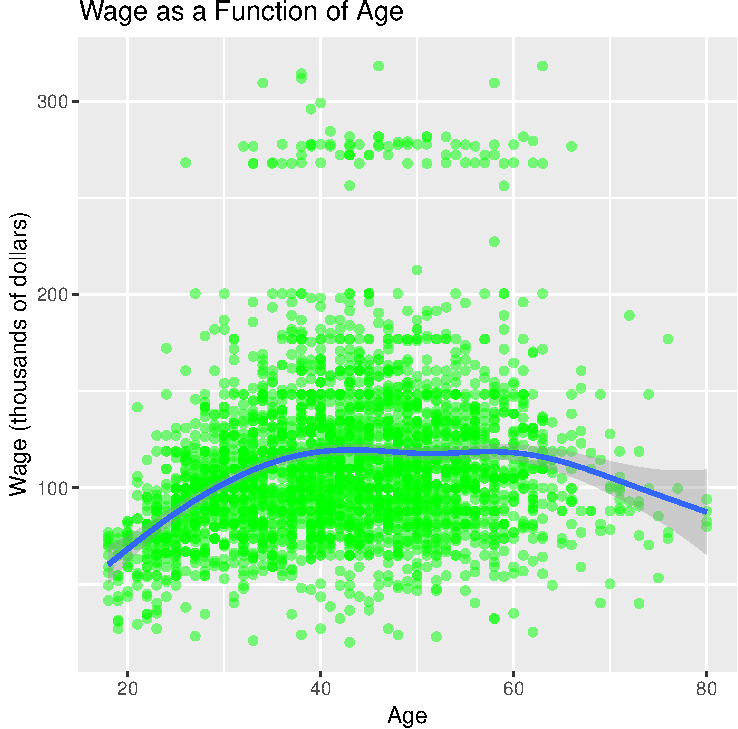
\includegraphics{homework1-handout_files/figure-latex/unnamed-chunk-11-1} \end{center}

There is a general pattern of increasing wage with age until it peaks in
the early 40s. After that there is a slight dip in wage until retirement
but it is generally a plateau until 62 after which point there is a more
clear decline after people have retired. Based on current knowledge of
trends in wage as a function of age and the justifications outlined
above, the shape of this graph is generally what would be expected.

\begin{verbatim}
#.  In this part of the problem, we will find a polynomial function of age that best fits the wage data.  For each polynomial function between $p=0, 1, 2, ... 10$:

    #.  Fit a linear regression to predict wages as a function of $age$, $age^2$, ... $age^p$ (you should include an intercept as well).  Note that $p=0$ model is an "intercept-only" model.
    
    #.  Use 5-fold cross validation to estimate the test error for this model. Save both the test error and the training error.  
\end{verbatim}

\begin{Shaded}
\begin{Highlighting}[]
\NormalTok{do.wage <-}\StringTok{ }\ControlFlowTok{function}\NormalTok{(chunkid, chunkdef, p, dat)\{}
\NormalTok{    Wage =}\StringTok{ }\NormalTok{dat}
\NormalTok{    train =}\StringTok{ }\NormalTok{(chunkdef }\OperatorTok{!=}\StringTok{ }\NormalTok{chunkid)}

    \ControlFlowTok{if}\NormalTok{(p}\OperatorTok{<}\DecValTok{1}\NormalTok{)\{}
\NormalTok{      predictors.df <-}\StringTok{ }\KeywordTok{data.frame}\NormalTok{(}\DataTypeTok{age0 =} \DecValTok{1}\NormalTok{)}
\NormalTok{      wage =}\StringTok{ }\KeywordTok{data.frame}\NormalTok{(Wage}\OperatorTok{$}\NormalTok{wage)}
      \KeywordTok{colnames}\NormalTok{(wage) =}\StringTok{ "wage"}
      
\NormalTok{      predictors_new =}\StringTok{ }\KeywordTok{cbind}\NormalTok{(predictors.df, wage)}
      
\NormalTok{      Xtr =}\StringTok{ }\NormalTok{predictors_new[train,}\DecValTok{1}\NormalTok{]  }\CommentTok{# get training set}
\NormalTok{      Ytr =}\StringTok{ }\NormalTok{predictors_new[train,}\DecValTok{2}\NormalTok{]  }\CommentTok{# get true response values in trainig set}
      
\NormalTok{      Xvl =}\StringTok{ }\KeywordTok{as.data.frame}\NormalTok{(predictors_new[}\OperatorTok{!}\NormalTok{train,}\DecValTok{1}\NormalTok{]) }\CommentTok{# get validation set}
      \KeywordTok{colnames}\NormalTok{(Xvl) <-}\StringTok{ }\KeywordTok{paste}\NormalTok{(}\StringTok{"age"}\NormalTok{, }\DecValTok{0}\NormalTok{, }\DataTypeTok{sep =} \StringTok{""}\NormalTok{)}
\NormalTok{      Yvl =}\StringTok{ }\NormalTok{predictors_new[}\OperatorTok{!}\NormalTok{train,}\DecValTok{2}\NormalTok{] }\CommentTok{# get true response values in validation set}
\NormalTok{    \}}\ControlFlowTok{else}\NormalTok{\{}
\NormalTok{      predictors <-}\StringTok{ }\KeywordTok{poly}\NormalTok{(Wage}\OperatorTok{$}\NormalTok{age, p, }\DataTypeTok{raw =} \OtherTok{TRUE}\NormalTok{)}
      
\NormalTok{      predictors.df <-}\StringTok{ }\KeywordTok{as.data.frame}\NormalTok{(predictors)}
      
      \KeywordTok{colnames}\NormalTok{(predictors.df) <-}\StringTok{ }\KeywordTok{paste}\NormalTok{(}\StringTok{"age"}\NormalTok{, }\DecValTok{1}\OperatorTok{:}\NormalTok{p, }\DataTypeTok{sep =} \StringTok{""}\NormalTok{)}
      
\NormalTok{      wage =}\StringTok{ }\KeywordTok{data.frame}\NormalTok{(Wage}\OperatorTok{$}\NormalTok{wage)}
      \KeywordTok{colnames}\NormalTok{(wage) =}\StringTok{ "wage"}
      
\NormalTok{      Xtr =}\StringTok{ }\NormalTok{predictors.df[train,}\DecValTok{1}\OperatorTok{:}\NormalTok{p]  }\CommentTok{# get training set}
\NormalTok{      Ytr =}\StringTok{ }\NormalTok{wage[train,}\DecValTok{1}\NormalTok{]  }\CommentTok{# get true response values in trainig set}

\NormalTok{      Xvl =}\StringTok{ }\KeywordTok{as.data.frame}\NormalTok{(predictors.df[}\OperatorTok{!}\NormalTok{train,}\DecValTok{1}\OperatorTok{:}\NormalTok{p]) }\CommentTok{# get validation set}
      \KeywordTok{colnames}\NormalTok{(Xvl) <-}\StringTok{ }\KeywordTok{paste}\NormalTok{(}\StringTok{"age"}\NormalTok{, }\DecValTok{1}\OperatorTok{:}\NormalTok{p, }\DataTypeTok{sep =} \StringTok{""}\NormalTok{)}
    
\NormalTok{      Yvl =}\StringTok{ }\NormalTok{wage[}\OperatorTok{!}\NormalTok{train,}\DecValTok{1}\NormalTok{] }\CommentTok{# get true response values in validation set}
      
\NormalTok{      predictors_new =}\StringTok{ }\KeywordTok{cbind}\NormalTok{(wage, predictors.df)}
      
\NormalTok{    \}}
\NormalTok{      lm.wage <-}\StringTok{ }\KeywordTok{lm}\NormalTok{(wage}\OperatorTok{~}\NormalTok{., }\DataTypeTok{data =}\NormalTok{ predictors_new)}
      
\NormalTok{      predYtr =}\StringTok{ }\KeywordTok{predict}\NormalTok{(lm.wage)  }\CommentTok{# predict training values}
\NormalTok{      predYvl =}\StringTok{ }\KeywordTok{predict}\NormalTok{(lm.wage,Xvl)  }\CommentTok{# predict validation values}
 
      \KeywordTok{data.frame}\NormalTok{(}\DataTypeTok{degree =}\NormalTok{ p,}
               \DataTypeTok{fold =}\NormalTok{ chunkid,}
               \DataTypeTok{train.error =} \KeywordTok{mean}\NormalTok{((predYtr }\OperatorTok{-}\StringTok{ }\NormalTok{Ytr)}\OperatorTok{^}\DecValTok{2}\NormalTok{), }\CommentTok{# compute and store train error}
               \DataTypeTok{val.error =} \KeywordTok{mean}\NormalTok{((predYvl }\OperatorTok{-}\StringTok{ }\NormalTok{Yvl)}\OperatorTok{^}\DecValTok{2}\NormalTok{)) }\CommentTok{# compute and store test error}
    

\NormalTok{\}}
\end{Highlighting}
\end{Shaded}

\begin{Shaded}
\begin{Highlighting}[]
\NormalTok{nfold =}\StringTok{ }\DecValTok{5}

\NormalTok{folds <-}\StringTok{ }\KeywordTok{cut}\NormalTok{(}\DecValTok{1}\OperatorTok{:}\DecValTok{3000}\NormalTok{, nfold, }\DataTypeTok{label =} \OtherTok{FALSE}\NormalTok{) }\OperatorTok\StringTok{ }
\StringTok{  }\KeywordTok{sample}\NormalTok{()}

\NormalTok{error.folds.wages =}\StringTok{ }\KeywordTok{data.frame}\NormalTok{()}

\NormalTok{allP =}\StringTok{ }\DecValTok{0}\OperatorTok{:}\DecValTok{10}

\KeywordTok{set.seed}\NormalTok{(}\DecValTok{5555}\NormalTok{)}

\ControlFlowTok{for}\NormalTok{ (j }\ControlFlowTok{in}\NormalTok{ allP)\{}
\NormalTok{  tmp.wage =}\StringTok{ }\KeywordTok{ldply}\NormalTok{(}\DecValTok{1}\OperatorTok{:}\NormalTok{nfold, do.wage,}
    \DataTypeTok{chunkdef=}\NormalTok{folds, }\DataTypeTok{p =}\NormalTok{ j, }\DataTypeTok{dat =}\NormalTok{ ISLR}\OperatorTok{::}\NormalTok{Wage)}
  
\NormalTok{  error.folds.wages =}\StringTok{ }\KeywordTok{rbind}\NormalTok{(error.folds.wages, tmp.wage)}
\NormalTok{\}}
\end{Highlighting}
\end{Shaded}

\begin{verbatim}
## Warning in predict.lm(lm.wage, Xvl): prediction from a rank-deficient fit
## may be misleading
\end{verbatim}

\begin{verbatim}
## Warning in predYtr - Ytr: longer object length is not a multiple of shorter
## object length
\end{verbatim}

\begin{verbatim}
## Warning in predict.lm(lm.wage, Xvl): prediction from a rank-deficient fit
## may be misleading
\end{verbatim}

\begin{verbatim}
## Warning in predYtr - Ytr: longer object length is not a multiple of shorter
## object length
\end{verbatim}

\begin{verbatim}
## Warning in predict.lm(lm.wage, Xvl): prediction from a rank-deficient fit
## may be misleading
\end{verbatim}

\begin{verbatim}
## Warning in predYtr - Ytr: longer object length is not a multiple of shorter
## object length
\end{verbatim}

\begin{verbatim}
## Warning in predict.lm(lm.wage, Xvl): prediction from a rank-deficient fit
## may be misleading
\end{verbatim}

\begin{verbatim}
## Warning in predYtr - Ytr: longer object length is not a multiple of shorter
## object length
\end{verbatim}

\begin{verbatim}
## Warning in predict.lm(lm.wage, Xvl): prediction from a rank-deficient fit
## may be misleading
\end{verbatim}

\begin{verbatim}
## Warning in predYtr - Ytr: longer object length is not a multiple of shorter
## object length

## Warning in predYtr - Ytr: longer object length is not a multiple of shorter
## object length

## Warning in predYtr - Ytr: longer object length is not a multiple of shorter
## object length

## Warning in predYtr - Ytr: longer object length is not a multiple of shorter
## object length

## Warning in predYtr - Ytr: longer object length is not a multiple of shorter
## object length

## Warning in predYtr - Ytr: longer object length is not a multiple of shorter
## object length

## Warning in predYtr - Ytr: longer object length is not a multiple of shorter
## object length

## Warning in predYtr - Ytr: longer object length is not a multiple of shorter
## object length

## Warning in predYtr - Ytr: longer object length is not a multiple of shorter
## object length

## Warning in predYtr - Ytr: longer object length is not a multiple of shorter
## object length

## Warning in predYtr - Ytr: longer object length is not a multiple of shorter
## object length

## Warning in predYtr - Ytr: longer object length is not a multiple of shorter
## object length

## Warning in predYtr - Ytr: longer object length is not a multiple of shorter
## object length

## Warning in predYtr - Ytr: longer object length is not a multiple of shorter
## object length

## Warning in predYtr - Ytr: longer object length is not a multiple of shorter
## object length

## Warning in predYtr - Ytr: longer object length is not a multiple of shorter
## object length

## Warning in predYtr - Ytr: longer object length is not a multiple of shorter
## object length

## Warning in predYtr - Ytr: longer object length is not a multiple of shorter
## object length

## Warning in predYtr - Ytr: longer object length is not a multiple of shorter
## object length

## Warning in predYtr - Ytr: longer object length is not a multiple of shorter
## object length

## Warning in predYtr - Ytr: longer object length is not a multiple of shorter
## object length

## Warning in predYtr - Ytr: longer object length is not a multiple of shorter
## object length

## Warning in predYtr - Ytr: longer object length is not a multiple of shorter
## object length

## Warning in predYtr - Ytr: longer object length is not a multiple of shorter
## object length

## Warning in predYtr - Ytr: longer object length is not a multiple of shorter
## object length

## Warning in predYtr - Ytr: longer object length is not a multiple of shorter
## object length

## Warning in predYtr - Ytr: longer object length is not a multiple of shorter
## object length

## Warning in predYtr - Ytr: longer object length is not a multiple of shorter
## object length

## Warning in predYtr - Ytr: longer object length is not a multiple of shorter
## object length

## Warning in predYtr - Ytr: longer object length is not a multiple of shorter
## object length

## Warning in predYtr - Ytr: longer object length is not a multiple of shorter
## object length

## Warning in predYtr - Ytr: longer object length is not a multiple of shorter
## object length

## Warning in predYtr - Ytr: longer object length is not a multiple of shorter
## object length

## Warning in predYtr - Ytr: longer object length is not a multiple of shorter
## object length

## Warning in predYtr - Ytr: longer object length is not a multiple of shorter
## object length

## Warning in predYtr - Ytr: longer object length is not a multiple of shorter
## object length

## Warning in predYtr - Ytr: longer object length is not a multiple of shorter
## object length

## Warning in predYtr - Ytr: longer object length is not a multiple of shorter
## object length

## Warning in predYtr - Ytr: longer object length is not a multiple of shorter
## object length

## Warning in predYtr - Ytr: longer object length is not a multiple of shorter
## object length

## Warning in predYtr - Ytr: longer object length is not a multiple of shorter
## object length

## Warning in predYtr - Ytr: longer object length is not a multiple of shorter
## object length

## Warning in predYtr - Ytr: longer object length is not a multiple of shorter
## object length

## Warning in predYtr - Ytr: longer object length is not a multiple of shorter
## object length

## Warning in predYtr - Ytr: longer object length is not a multiple of shorter
## object length

## Warning in predYtr - Ytr: longer object length is not a multiple of shorter
## object length

## Warning in predYtr - Ytr: longer object length is not a multiple of shorter
## object length

## Warning in predYtr - Ytr: longer object length is not a multiple of shorter
## object length

## Warning in predYtr - Ytr: longer object length is not a multiple of shorter
## object length

## Warning in predYtr - Ytr: longer object length is not a multiple of shorter
## object length

## Warning in predYtr - Ytr: longer object length is not a multiple of shorter
## object length
\end{verbatim}

\begin{Shaded}
\begin{Highlighting}[]
\NormalTok{error.folds.wages}
\end{Highlighting}
\end{Shaded}

\begin{verbatim}
##    degree fold train.error val.error
## 1       0    1    1760.658  1818.650
## 2       0    2    1614.991  2287.384
## 3       0    3    1826.166  1596.636
## 4       0    4    1798.015  1574.150
## 5       0    5    1863.495  1426.657
## 6       1    1    1827.774  1750.271
## 7       1    2    1655.951  2223.948
## 8       1    3    1901.422  1519.542
## 9       1    4    1880.733  1516.942
## 10      1    5    1901.815  1359.657
## 11      2    1    1907.899  1678.454
## 12      2    2    1743.568  2096.245
## 13      2    3    1976.139  1442.519
## 14      2    4    1980.702  1478.615
## 15      2    5    1981.440  1293.218
## 16      3    1    1911.754  1674.902
## 17      3    2    1747.873  2084.869
## 18      3    3    1981.488  1437.902
## 19      3    4    1986.530  1477.805
## 20      3    5    1987.110  1287.313
## 21      4    1    1915.649  1666.621
## 22      4    2    1748.719  2086.505
## 23      4    3    1983.835  1440.968
## 24      4    4    1988.344  1476.949
## 25      4    5    1991.093  1281.631
## 26      5    1    1916.859  1665.437
## 27      5    2    1748.616  2082.571
## 28      5    3    1985.084  1440.281
## 29      5    4    1986.945  1479.105
## 30      5    5    1993.047  1283.141
## 31      6    1    1916.029  1661.778
## 32      6    2    1750.702  2083.477
## 33      6    3    1984.943  1438.353
## 34      6    4    1989.868  1479.196
## 35      6    5    1996.814  1281.178
## 36      7    1    1917.749  1660.059
## 37      7    2    1751.579  2075.054
## 38      7    3    1983.546  1440.512
## 39      7    4    1991.902  1482.062
## 40      7    5    2000.021  1282.036
## 41      8    1    1918.110  1660.774
## 42      8    2    1751.449  2075.277
## 43      8    3    1984.295  1440.392
## 44      8    4    1991.731  1481.545
## 45      8    5    1999.785  1281.525
## 46      9    1    1918.572  1657.291
## 47      9    2    1752.903  2068.092
## 48      9    3    1984.543  1446.357
## 49      9    4    1992.879  1480.893
## 50      9    5    2002.558  1275.206
## 51     10    1    1918.611  1657.311
## 52     10    2    1753.028  2068.021
## 53     10    3    1984.496  1446.474
## 54     10    4    1992.864  1480.923
## 55     10    5    2002.577  1275.105
\end{verbatim}

\begin{Shaded}
\begin{Highlighting}[]
\NormalTok{error.means =}\StringTok{ }\KeywordTok{aggregate}\NormalTok{(error.folds.wages[, }\DecValTok{3}\OperatorTok{:}\DecValTok{4}\NormalTok{], }\KeywordTok{list}\NormalTok{(error.folds.wages}\OperatorTok{$}\NormalTok{degree), mean)}
\KeywordTok{colnames}\NormalTok{(error.means) =}\StringTok{ }\KeywordTok{c}\NormalTok{(}\StringTok{"degree"}\NormalTok{, }\StringTok{"Training Error"}\NormalTok{,}\StringTok{"Validation Error"}\NormalTok{)}

\NormalTok{error.melt =}\StringTok{ }\KeywordTok{melt}\NormalTok{(error.means, }\DataTypeTok{id.vars=}\KeywordTok{c}\NormalTok{(}\StringTok{'degree'}\NormalTok{), }\DataTypeTok{value.name=}\StringTok{'error'}\NormalTok{)}
\end{Highlighting}
\end{Shaded}

\begin{verbatim}
#. Plot both the test error and training error (on the same plot) for each of the models estimated above as a function of $p$.  What do you observe about the training error as $p$ increases? What about the test error? Based on your results, which model should you select and why?
\end{verbatim}

\begin{Shaded}
\begin{Highlighting}[]
\NormalTok{wage.error.plot <-}\StringTok{ }\KeywordTok{ggplot}\NormalTok{(error.melt, }\KeywordTok{aes}\NormalTok{(}\DataTypeTok{x=}\NormalTok{degree, }\DataTypeTok{y=}\NormalTok{error, }\DataTypeTok{col =}\NormalTok{ variable))}\OperatorTok{+}\StringTok{ }
\StringTok{    }\KeywordTok{geom_line}\NormalTok{() }\OperatorTok{+}
\StringTok{    }\KeywordTok{stat_summary}\NormalTok{(}\KeywordTok{aes}\NormalTok{(}\DataTypeTok{group=}\NormalTok{variable), }\DataTypeTok{fun.y=}\StringTok{"mean"}\NormalTok{, }\DataTypeTok{geom=}\StringTok{'line'}\NormalTok{, }\DataTypeTok{size=}\DecValTok{2}\NormalTok{) }\OperatorTok{+}
\StringTok{    }\KeywordTok{scale_x_continuous}\NormalTok{(}\DataTypeTok{breaks =} \KeywordTok{seq}\NormalTok{(}\DecValTok{0}\NormalTok{,}\DecValTok{10}\NormalTok{, }\DataTypeTok{by =} \DecValTok{1}\NormalTok{)) }\OperatorTok{+}
\StringTok{    }\KeywordTok{xlab}\NormalTok{(}\StringTok{"Degree"}\NormalTok{) }\OperatorTok{+}\StringTok{ }\KeywordTok{ylab}\NormalTok{(}\StringTok{"Error"}\NormalTok{) }\OperatorTok{+}\StringTok{ }
\StringTok{    }\KeywordTok{ggtitle}\NormalTok{(}\StringTok{"Error for Various Degree Polynomial Models for Wage as a Function of Age"}\NormalTok{) }\OperatorTok{+}\StringTok{ }
\StringTok{    }\KeywordTok{theme}\NormalTok{(}\DataTypeTok{plot.title =} \KeywordTok{element_text}\NormalTok{(}\DataTypeTok{hjust =} \FloatTok{0.5}\NormalTok{))}
    

\NormalTok{wage.error.plot}
\end{Highlighting}
\end{Shaded}

\begin{center}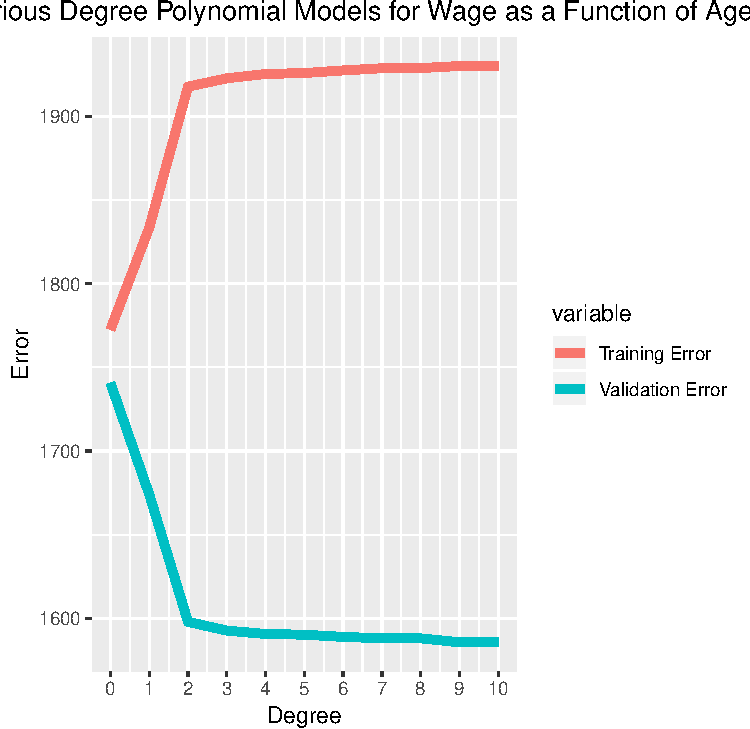
\includegraphics{homework1-handout_files/figure-latex/unnamed-chunk-15-1} \end{center}

As the degree (p) of the polynomial model used increases, the training
error increases. For the first three degrees (0 through 2), there's a
rapid increase in training error and then there is a slightly greater
increase to p = 4 before it plateaus with only a slightly further
increase as the degree of the polynomial model approaches 10. A similar
pattern except in the decreasing direction is observed for the
validation error with a rapid decrease in validation error from p = 0 to
2 and then a gradual decrease in validation error to p = 4 and minimal
change as the degree of the model goes to p = 10. Based on these
results, the fourth degree polynomial should be selected because it has
a low validation error similar to higher degree polynomials and the
training error has yet to increase much more. At p = 0 through 3, the
model is not flexible enough and will have a higher bias. Choosing a
higher degree polynomial model than p = 4 won't make much difference in
improving the model's validation error and the training error will also
increase. While selecting a higher degree polynomial would increase
flexibility of the model, it may result in overfitting with higher
variance in modeled results. Additionally, a polynomial degree 4 would
have a generally parabolic shape with slightly greater flexibility,
which is generally the shape that might be expected to describe wage as
a function of age (increase in pay until a peak age where there is a
plateau and then a gradual drop off). Given these concerns, a fourth
degree polynomial model seems most appropriate for this scenario.

\begin{verbatim}
  Note: `poly(age, degree=p, raw=TRUE)` will return a matrix with $p$ columns, where the $p$-th column is $age^p$.  For the predictors in your regression use `poly(age, degree=p, raw=FALSE)`.  The `raw=FALSE` option returns predictors which are numerically more stable (it returns a matrix of "orthogonal polynomials").  Numerical stability can be an issue because $age^p$ can be very very large if $p$ is large.  The orthogonal polynomials returned when `raw=FALSE` are rescaled to account for this so please use the `raw=FALSE` option.   
  Hint: A function similar to `do.chunk` from problem 4 will be helpful here as well.   
    
\end{verbatim}

\begin{center}\rule{0.5\linewidth}{\linethickness}\end{center}

\begin{enumerate}
\def\labelenumi{\arabic{enumi}.}
\setcounter{enumi}{6}
\item
  \textbf{(231 Only)} \textbf{The bias-variance tradeoff}. Prove that
  the mean squared error can be decomposed into the variance plus bias
  squared. That is, who
  \(E[(\hat \theta - \theta)^2] = \text{Var}(\hat \theta) + \text{Bias}(\hat \theta )^2\)
  where \(\text{Bias}(\hat \theta) = E[\hat \theta - \theta]\). Here
  \(\hat \theta\) is an estimator (a random variable) of the fixed
  unknown constant \(\theta\). Hint: reogranize terms in the MSE by
  adding and subtracting \(E[\hat \theta]\).
\item
  \textbf{(231 Only)} As we discussed in class, distance metrics satisfy
  the following properties:

  \begin{itemize}
  \item
    \emph{Positivity}:

    \begin{itemize}
    \tightlist
    \item
      \(d(x,y)\geq 0\)
    \item
      \(d(x,y) = 0\) only if \(x=y\)
    \end{itemize}
  \item
    \emph{Symmetry}:

    \begin{itemize}
    \tightlist
    \item
      \(d(x,y) = d(y,x)\) for all \(x\) and \(y\)
    \end{itemize}
  \item
    \emph{Triangle Inequality}:

    \begin{itemize}
    \tightlist
    \item
      \(d(x,z) \leq d(x,y) + d(y,z)\) for \(x,\ y,\text{ and } z\)
    \end{itemize}
  \end{itemize}

  Show that the following measures are distance metrics by showing the
  above properties hold:

  \begin{enumerate}
  \item
    \(d(x,y) = \|x-y\|_2\)
  \item
    \(d(x,y) = \|x-y\|_\infty\)
  \end{enumerate}
\end{enumerate}


\end{document}
